\documentclass[tikz,border=2pt]{standalone}
\usepackage{pgfplots}
\pgfplotsset{compat=1.18}
\usetikzlibrary{positioning}
\usepackage{helvet}
\renewcommand{\familydefault}{\sfdefault}
\definecolor{ieeecolor}{HTML}{042C53}
\definecolor{jrnlcolor}{HTML}{378ADD}
\definecolor{othercolor}{HTML}{B4B2A9}
\definecolor{confcolor}{HTML}{D98B3F}
\begin{document}
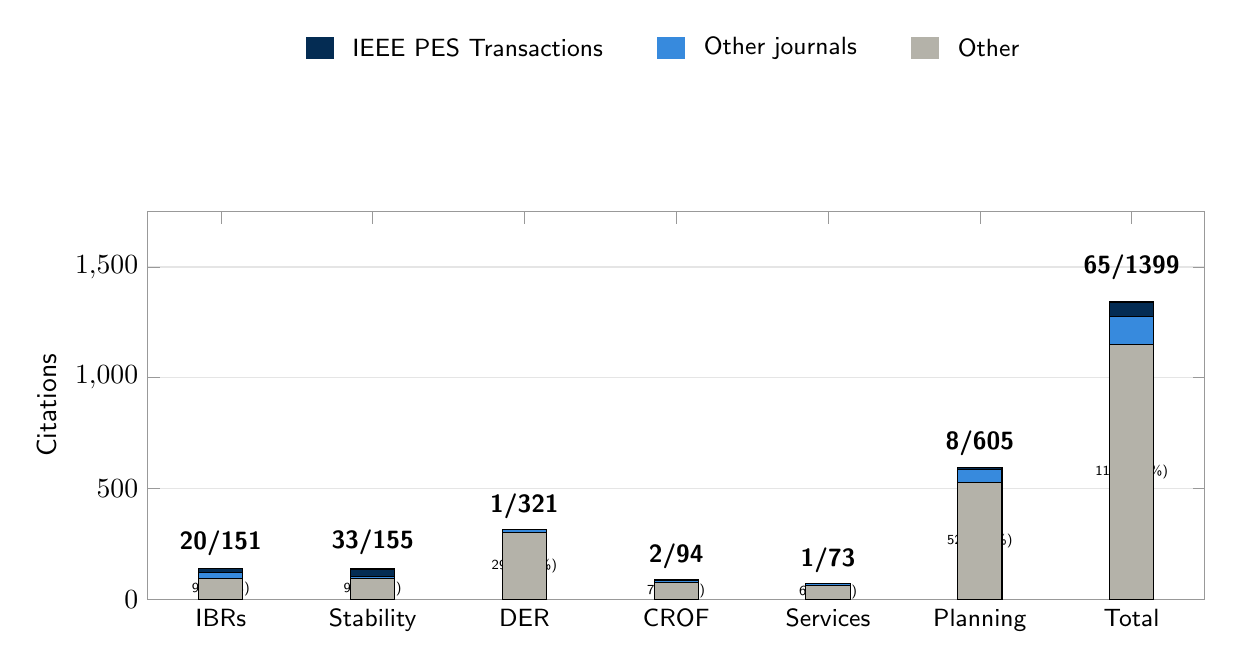
\begin{tikzpicture}
\begin{axis}[
    ybar stacked, bar width=16pt,
    width=15cm, height=6.5cm,
    symbolic x coords={IBRs,Stability,DER,CROF,Services,Planning,Total},
    xtick=data,
    x tick label style={font=\small},
    ylabel={Citations},
    ymin=0, ymax=1749,
    axis line style={color=black!40},
    tick style={color=black!40},
    ymajorgrids, grid style={color=black!10},
    enlarge x limits=0.08,
]
\addplot[fill=othercolor] coordinates {(IBRs,94) (Stability,93) (DER,299) (CROF,77) (Services,60) (Planning,528) (Total,1151)};
\addplot[fill=jrnlcolor] coordinates {(IBRs,25) (Stability,10) (DER,15) (CROF,9) (Services,9) (Planning,58) (Total,126)};
\addplot[fill=ieeecolor] coordinates {(IBRs,20) (Stability,33) (DER,1) (CROF,2) (Services,1) (Planning,8) (Total,65)};
\node[font=\tiny, text=black] at (axis cs:IBRs,47.0) {94 (62\%)};
\node[font=\tiny, text=white] at (axis cs:IBRs,106.5) {25 (17\%)};
\node[font=\tiny, text=white] at (axis cs:IBRs,129.0) {20 (13\%)};
\node[font=\small\bfseries, anchor=south] at (axis cs:IBRs,151) {20/151};
\node[font=\tiny, text=black] at (axis cs:Stability,46.5) {93 (60\%)};
\node[font=\tiny, text=white] at (axis cs:Stability,98.0) {10 (6\%)};
\node[font=\tiny, text=white] at (axis cs:Stability,119.5) {33 (21\%)};
\node[font=\small\bfseries, anchor=south] at (axis cs:Stability,155) {33/155};
\node[font=\tiny, text=black] at (axis cs:DER,149.5) {299 (93\%)};
\node[font=\small\bfseries, anchor=south] at (axis cs:DER,321) {1/321};
\node[font=\tiny, text=black] at (axis cs:CROF,38.5) {77 (82\%)};
\node[font=\tiny, text=white] at (axis cs:CROF,81.5) {9 (10\%)};
\node[font=\small\bfseries, anchor=south] at (axis cs:CROF,94) {2/94};
\node[font=\tiny, text=black] at (axis cs:Services,30.0) {60 (82\%)};
\node[font=\tiny, text=white] at (axis cs:Services,64.5) {9 (12\%)};
\node[font=\small\bfseries, anchor=south] at (axis cs:Services,73) {1/73};
\node[font=\tiny, text=black] at (axis cs:Planning,264.0) {528 (87\%)};
\node[font=\tiny, text=white] at (axis cs:Planning,557.0) {58 (10\%)};
\node[font=\small\bfseries, anchor=south] at (axis cs:Planning,605) {8/605};
\node[font=\tiny, text=black] at (axis cs:Total,575.5) {1151 (82\%)};
\node[font=\tiny, text=white] at (axis cs:Total,1214.0) {126 (9\%)};
\node[font=\small\bfseries, anchor=south] at (axis cs:Total,1399) {65/1399};
\end{axis}
\begin{scope}[shift={(2.0,7.0)}]
\node[fill=ieeecolor, minimum width=10pt, minimum height=8pt, anchor=west] (legbox0) at (0,0) {}; \node[anchor=west, font=\small, right=3pt of legbox0] (legtxt0) {IEEE PES Transactions}; \node[fill=jrnlcolor, minimum width=10pt, minimum height=8pt, anchor=west, right=16pt of legtxt0] (legbox1) {}; \node[anchor=west, font=\small, right=3pt of legbox1] (legtxt1) {Other journals}; \node[fill=othercolor, minimum width=10pt, minimum height=8pt, anchor=west, right=16pt of legtxt1] (legbox2) {}; \node[anchor=west, font=\small, right=3pt of legbox2] (legtxt2) {Other};
\end{scope}
\end{tikzpicture}
\end{document}
